% Paquets généraux
\documentclass[a4paper,12pt,titlepage,twoside]{article}
\usepackage[T1]{fontenc}
\usepackage[utf8]{inputenc}
\usepackage[french]{babel}
\usepackage{subcaption}
\addto\captionsfrench{%
  \renewcommand{\tablename}{Tableau}%
}
\usepackage[gen]{eurosym}
%\usepackage[dvips]{graphicx}
\usepackage{minted}
\usepackage{fancyhdr}
\usepackage{pdfpages} 
\usepackage{multido}
\usepackage{hyperref}
\usepackage{textcomp}
\usepackage{schemabloc}
%\usepackage[bitstream-charter]{mathdesign}
\usepackage{array}
\newcolumntype{P}[1]{>{\centering\arraybackslash}p{#1}}
\usepackage[shortlabels]{enumitem}
\usepackage[framemethod=TikZ]{mdframed}

\newcommand{\id}{30}
\newcommand{\nom}{Calculs d'hyperstatisme}
\newcommand{\sequence}{04}
\newcommand{\nomsequence}{Liaisons entre les solides}
\newcommand{\num}{03}
\newcommand{\type}{TD}
\newcommand{\descrip}{En appliquant les règles de la théorie des mécanisme, déterminer le degré d'hyperstatisme de plusieurs systèmes et proposer des solutions afin de diminuer ce degré}
\newcommand{\competences}{B2-12: Proposer une modélisation des liaisons avec leurs caractéristiques géométriques. \\ &  B2-13: Proposer un modèle cinématique paramétré à partir d'un système réel, d'une maquette numérique ou d'u \\ &  B2-17: Simplifier un modèle de mécanisme. \\ &  B2-18: Modifier un modèle pour le rendre isostatique.}
\newcommand{\nbcomp}{4}
\newcommand{\systemes}{E.P.A.S, Machine d'essai de traction}
\newcommand{\systemesnum}{14, 13}
\newcommand{\systemessansaccent}{E.P.A.S, Machine d'essai de traction}
\newcommand{\ilot}{3}
\newcommand{\ilotstr}{03}
\newcommand{\dossierilot}{\detokenize{Ilot_03 E.P.A.S, Machine d'essai de traction}}
\newcommand{\imageun}{EPAS}
\newcommand{\imagedeux}{Machine_dessai_de_traction}

%\usepackage{style}
\usepackage{bodegraph}
\usepackage{rpcinematik}
\usepackage[locale = FR]{siunitx}
\usepackage{caption}
\newcommand{\institute}{Lycée Dorian}
\usepackage{calc}

\usepackage{listings}
\usepackage{fancyvrb}
\usepackage{color}
\usepackage{xcolor}
\usepackage{colortbl}
\usepackage{helvet}
\usepackage[frenchmath]{newtxsf} % for sans serif symbols
\renewcommand{\familydefault}{\sfdefault}
%\usepackage{amsfonts}
%\usepackage{amsmath}
%\usepackage{lmodern}
\usepackage{mathastext}
%\usepackage{xspace}
\usepackage{varioref}
\usepackage{tabularx}
%\usepackage{floatflt}
\usepackage{graphics}
\usepackage{wrapfig}
\usepackage{textcomp}
\usepackage{tikz,tkz-tab}
\usepackage[european resistor, european voltage, european current]{circuitikz}
\usepackage{wrapfig}
\usepackage{gensymb}
\usepackage[percent]{overpic}
\usetikzlibrary{babel}
\usepackage{ifthen}
\usepackage{cancel}
\usepackage{etoolbox}
\usepackage{multirow}
%\usepackage{boxedminipage}
\definecolor{gris25}{gray}{0.75}
\definecolor{bleu}{RGB}{18,33,98}
\definecolor{bleuf}{RGB}{42,94,171}
\definecolor{bleuc}{RGB}{231,239,247}
\definecolor{bleum}{RGB}{160,195,226}
\definecolor{rougef}{RGB}{185,18,27}
\definecolor{rougec}{RGB}{255,188,204}%255,230,231
\definecolor{vertf}{RGB}{103,126,82}
\definecolor{vertc}{RGB}{220,255,191}
\definecolor{forestgreen}{rgb}{0.13,0.54,0.13}
\definecolor{blcr}{rgb}{0.59,0.69,0.84}
\definecolor{blfr}{rgb}{0.32,0.51,0.75}
\definecolor{orfr}{rgb}{0.90,0.42,0.15}
\definecolor{orcr}{rgb}{0.90,0.65,0.50}
\definecolor{orangef}{rgb}{0.659,0.269,0.072}
\definecolor{orange}{rgb}{0.58,0.35,0.063}
\definecolor{orangec}{rgb}{0.43,0.32,0.25}
\definecolor{rcorrect}{rgb}{0.6,0,0}
\definecolor{sequence}{rgb}{0.75,0.75,0.75}
\definecolor{competences}{rgb}{0.61,0.73,0.35}
\definecolor{rose}{HTML}{ff00ff}
\definecolor{grisf}{HTML}{222222}
\definecolor{grisc}{HTML}{636363}
\definecolor{normal}{HTML}{4087c4}
\definecolor{info}{HTML}{5bc0de}
\definecolor{success}{RGB}{92,184,92}
\definecolor{warning}{RGB}{240,173,78}
\definecolor{danger}{RGB}{217,83,79}
\hypersetup{                    % parametrage des hyperliens
    colorlinks=true,                % colorise les liens
    breaklinks=true,                % permet les retours à la ligne pour les liens trop longs
    urlcolor= blfr,                 % couleur des hyperliens
    linkcolor= orange,                % couleur des liens internes aux documents (index, figures, tableaux, equations,...)
    citecolor= forestgreen                % couleur des liens vers les references bibliographiques
    }

\newcolumntype{M}[1]{>{\centering\arraybackslash}m{#1}}
\definecolor{codegreen}{rgb}{0,0.6,0}
\definecolor{codegray}{rgb}{0.5,0.5,0.5}
\definecolor{codepurple}{rgb}{0.58,0,0.82}
\definecolor{backcolour}{rgb}{0.95,0.95,0.92}

\lstdefinestyle{mystyle}{
    backgroundcolor=\color{backcolour},   
    commentstyle=\color{codegreen},
    keywordstyle=\color{magenta},
    numberstyle=\tiny\color{codegray},
    stringstyle=\color{codepurple},
    basicstyle=\ttfamily\footnotesize,
    breakatwhitespace=false,         
    breaklines=true,                 
    captionpos=b,                    
    keepspaces=true,                 
    numbers=left,                    
    numbersep=5pt,                  
    showspaces=false,                
    showstringspaces=false,
    showtabs=false,                  
    tabsize=2
}

\lstset{style=mystyle}

% Mise en page
\pagestyle{fancy}

\setlength{\hoffset}{-18pt}
\setlength{\oddsidemargin}{0pt} 	% Marge gauche sur pages impaire2s
\setlength{\evensidemargin}{0pt} 	% Marge gauche sur pages paires
\setlength{\marginparwidth}{00pt} 	% Largeur de note dans la marge
\setlength{\headwidth}{481pt} 	 	% Largeur de la zone de tête (17cm)
\setlength{\textwidth}{481pt} 	 	% Largeu\textbf{r de la zone de texte (17cm)
\setlength{\voffset}{-18pt} 		% Bon pour DOS
\setlength{\marginparsep}{7pt}	 	% Séparation de la marge
\setlength{\topmargin}{-30pt} 		% Pas de marge en haut
\setlength{\headheight}{55pt} 		% Haut de page
\setlength{\headsep}{20pt} 		% Entre le haut de page et le texte
\setlength{\footskip}{30pt} 		% Bas de\textbf{ page + séparation
\setlength{\textheight}{700pt} 		% Hauteur de l'icone zone de texte (25cm)
\setlength\fboxrule{1 pt}
\renewcommand{\baselinestretch}{1}
\setcounter{tocdepth}{1}
\newcommand{\cadre}[2]
{\fbox{
  \begin{minipage}{#1\linewidth}
   \begin{center}
    #2\\
   \end{center}
  \end{minipage}
 }
}

\newcommand{\repon}[1]
{
~\ \\
\begin{tabular}{|m{\linewidth}|}
 \hline
\multido{}{#1}{\\ \hline}
\end{tabular}
}


\newcommand{\objectif}[1]{
\mdfsetup{%
frametitle={%
\tikz[baseline=(current bounding box.east),outer sep=0pt]
\node[anchor=east,rectangle,fill=bleum]
{\strut Objectif~};}}
\mdfsetup{innertopmargin=10pt,linecolor=bleum,%
linewidth=2pt,topline=true,%
frametitleaboveskip=\dimexpr-\ht\strutbox\relax
}
\begin{mdframed}[]\relax%
#1
\end{mdframed}}


\newcounter{num_quest} \setcounter{num_quest}{0}
\newcounter{num_rep} \setcounter{num_rep}{0}
\newcounter{num_cor} \setcounter{num_cor}{0}

\newcommand{\feuilleDR}[1]{
	\begin{tikzpicture}
		\draw[gray!30](0,0)grid[step=0.5cm](\linewidth,#1);
	\end{tikzpicture}
}

%\newcommand{\question}[1]{\refstepcounter{num_quest}\par
%~\ \\ \parbox[t][][t]{0.15\linewidth}{\textbf{Question \arabic{num_quest}}}\parbox[t][][t]{0.85\linewidth}{#1\label{q\the\value{num_quest}}}\par
%}

\newcommand{\question}[1]{\refstepcounter{num_quest}\par
~\ \\ \textbf{Question \arabic{num_quest} : }#1\label{q\the\value{num_quest}}\par
}

\newcommand{\posetafigure}[3]{
\begin{figure}[ht!]
 \begin{center}
  \includegraphics[width=#2\linewidth]{img/#1}
 \end{center}
 \caption{\label{#1} #3}
\end{figure}}

\newcommand{\goforum}{
\begin{figure}

\end{figure}
\begin{center}
 \includegraphics[width=0.7\linewidth]{../../../img/go_forum}
\end{center}
\label{go_forum}
\caption{J'pète les plombs}
\end{figure}}

\newcommand{\reponse}[4][1]
{\noindent
\parbox{\textwidth}{
\rule{\linewidth}{.5pt}\\
\textbf{Question\ifthenelse{#1>1}{s}{} \multido{}{#1}{%
\refstepcounter{num_rep}\ref{q\the\value{num_rep}} }:} ~\ \\
\ifdef{\public}{#3 \ifthenelse{#2>0}{~\ \\ 	\feuilleDR{#2}}}{#4}
}}

\newboolean{printdr}
\newboolean{printcor}
\setboolean{printdr}{false}
\setboolean{printcor}{false}

\newcommand{\reponseinfo}[2][1]
{\noindent
\rule{\linewidth}{.5pt}\\
\textbf{Question\ifthenelse{#1>1}{s}{} \multido{}{#1}{%
\refstepcounter{num_rep}\ref{q\the\value{num_rep}} }:} ~\ \\
\ifdef{\public}{\parbox{\textwidth}{\ifthenelse{#2>0}{~\ \\ 	\feuilleDR{#2}}}
\setboolean{printdr}{true}\setboolean{printcor}{false}}
{\setboolean{printdr}{false}\setboolean{printcor}{true}}
}

\makeatletter
\newcommand\modulo[2]{
    \newcounter{lastpagesujet}
	\setcounter{lastpagesujet}{#1}
    \divide\value{lastpagesujet} by #2
    \multiply\value{lastpagesujet} by #2
    \advance\value{lastpagesujet} by #2
    \advance\value{lastpagesujet} by 1\relax
    }
\makeatother

\newcommand{\finsujet}[1]
{
    \begin{center}
    \Large{FIN}
    \end{center}
        
    \ifthenelse{\equal{#1}{public}}{\def\public{}}{}

	\newpage

}

\newcommand{\debutcor}
{	
    \ifdef{\public}{
    	\modulo{\value{page}-1}{4}
		\whiledo{\value{page}<\value{lastpagesujet}}{~\ \newpage}
        \pagestyle{docreponse}
	}{\pagestyle{correction}}

    \ifdef{\public}{
        \begin{tikzpicture} 
            \draw (0,0) rectangle (2,2);
            \draw (0,0) -- (2,2);
            \draw (1.5,0.5) node {\large 20};
            \draw (2.5,0) rectangle (16,2);
            \draw (4.5,1.7) node {\large Commentaires:};
        \end{tikzpicture}
    }
    ~\ \\
}

%\newcommand{\repcarre}[2]
%{
%~\ \\
%\begin{tikzpicture}
%\draw [fill=white] (0,0) rectangle +(\linewidth,#1);
%\node[align=left] at (1.1,#2-0.3) {\textbf{Question #1:}};
%\end{tikzpicture}
%}

\newcommand{\titre}[1]
{\begin{center}
\cadre{0.8}{\huge #1} 
\end{center}
}


%Définition des torseurs :
\newcommand{\torseur}[2]{\left\{\mathcal{#1}_{#2} \right\}}
\newcommand{\torseurh}[3]{\left\{\genfrac{}{}{0pt}{0}{#1}{#2}\right\}_{#3}}
\newcommand{\torseurv}[8]{\left\{
\begin{matrix}
#1 & #4 \\ #2 & #5 \\ #3 &#6
\end{matrix}
\right\}_{{#7},{#8}}}

%Définition des torseurs :
%\newcommand{\torseur}[2]{\left \{\mbox{\relsize{2}{$\mathcal {#1}$}\relsize{-2}}\phantom{}_{\mbox{\scriptsize $#2$}} \right \}}
%\newcommand{\torseurh}[3]{\left\{\genfrac{}{}{0pt}{0}{#1}{#2}\right\}_{#3}}
%\newcommand{\torseurv}[8]{
%\left\{\begin{array}{@{}c|c@{}} #1 & #4 \\ #2 & #5 \\ #3 & #6 \end{array} \right\}_{#7,#8}
%}
\newcommand{\derivee}[2]{\left.\dfrac{\d #1}{\d t}\right|_{#2}}
\newcommand{\tripleint}{\int\!\!\!\!\!\int\!\!\!\!\!\int}

% Notation cinématique et statique
\newcommand{\cinematique}[2]{\mbox{#1}/\mbox{#2}}
\newcommand{\statique}[2]{\mbox{#1}\rightarrow\mbox{#2}}
\newcommand{\moment}[3]{\vv {#1}_{\scriptsize{#3}}(#2)}
\newcommand{\resultante}[2]{\vv {#1}_{\scriptsize{#2}}}


%Commande de base
\newcommand{\jo}{\left(j\omega\right)} % j \omega dans l'analyse fréquentielle
\newcommand{\tl}{\xrightarrow{\mathcal{L}}} % transformée de laplace sur fleche
\newcommand{\tli}{\xrightarrow{\mathcal{L}^{-1}}} % transformée inverse de laplace sur fleche
\renewcommand{\d}[1][]{\mathrm{d#1}}
\newcommand{\dd}[1][]{\mathrm{d#1}}
\newcommand{\vect}[2]{{#1}\wedge{#2}}
\newcommand{\base}[3]{(\vec #1,\vec #2,\vec #3)}
\newcommand{\vectbase}[4]{{\vphantom{\left| \begin{matrix}
#1\\#2\\#3 \end{matrix} \right|}}_{#4}{\left| \begin{matrix}
#1\\#2\\#3 \end{matrix} \right.}}
%Pour avoir les paragraphes sous la forme I, II, III
\renewcommand{\thesection}{\Roman{section}}
\setcounter{secnumdepth}{3}
\renewcommand{\Frlabelitemii}{$\bullet$}

% En tête et pied de page
\lhead{\nom}
\rhead{\includegraphics[width=2cm]{../../../img/logo}}
\lfoot{\auteurun,\ \auteurdeux}
\cfoot{Page \thepage}

\fancypagestyle{docreponse}{%
  \fancyhf{}
  \fancyhead[LO]{NOM Prénom: .............................}
  \rhead{\includegraphics[width=2cm]{../../../img/logo}\hspace{2pt}}
  \ifdef{\auteurdeux}{\lfoot{\auteurun,\ \auteurdeux}}{\lfoot{\auteurun}}
  \rfoot{\nom}
  \lfoot{Document réponse}
  \cfoot{Page \thepage}
   }

\fancypagestyle{correction}{%
  \fancyhf{}
  \lhead{\colorbox{danger}{\begin{minipage}{0.65\paperwidth} \textcolor{white}{\textbf{Correction}} \end{minipage}} }
  \rhead{\includegraphics[width=2cm]{../../../img/logo}}
  \lfoot{Renaud Costadoat, Françoise Puig}
  \rfoot{\colorbox{danger}{\begin{minipage}{0.3\paperwidth} \begin{flushright}\textcolor{white}{\textbf{Correction}}\end{flushright} \end{minipage}} }
  \cfoot{Page \thepage}
}

\fancypagestyle{correctioninfo}{%
  \fancyhf{}
  \lhead{\colorbox{danger}{\begin{minipage}{0.65\paperwidth} \textcolor{white}{\textbf{Correction}} \end{minipage}} }
  \rhead{\includegraphics[width=2cm]{../../../img/logo}}
  \lfoot{Renaud Costadoat, Juliette Genzmer}
  \rfoot{\colorbox{danger}{\begin{minipage}{0.6\paperwidth} \begin{flushright}\textcolor{white}{\textbf{Correction}}\end{flushright} \end{minipage}} }}

\renewcommand{\footrulewidth}{0.4pt}

\usepackage{eso-pic}
\newcommand{\BackgroundPic}{%
\put(0,0){%
\parbox[b][\paperheight]{\paperwidth}{%
\vfill
\begin{center}
\hspace{0.5cm}\vspace{0.5cm}
\includegraphics[width=\paperwidth,height=\paperheight,%
keepaspectratio]{../../../img/fond3}%
\end{center}
\vfill
}}}

\newcommand{\BackgroundPicdeux}{%
\put(25,-30){%
\parbox[b][\paperheight]{\paperwidth}{%
\vfill
\begin{center}
\includegraphics[width=\paperwidth,height=\paperheight,%
keepaspectratio]{../../../img/fond4}%
\end{center}
\vfill
}}}

\begin{document}

\pagestyle{empty}

\AddToShipoutPicture*{\BackgroundPic}

\includegraphics[width=2cm]{../../../img/logo}

\Huge{DS \numero - \sujet}

\vspace{1cm}

\ifdef{\prive}{\begin{center}\colorbox{danger}{\Huge{Avec Correction}}\end{center}}{}

\begin{center}
\centering\huge{PTSI}
\end{center}

\vspace{2cm}


\begin{center}
\centering\Large{\jour}
\end{center}

\vspace{2cm}

\normalsize

\tableofcontents

\newpage

\AddToShipoutPicture{\BackgroundPicdeux}

\pagestyle{fancy}

\begin{center}
\Huge \sujet
\end{center}


\normalsize


\section{Exercice de cours}

\question{Écrire une relation de champs de vecteurs vitesse (Varignon), dans le mouvement de 1/0, entre les points A et B.}

\question{Écrire le torseur d’une liaison pivot d’axe (A,$\overrightarrow{x}$) en ligne et en colonne dans la base $(\overrightarrow{x},\overrightarrow{y},\overrightarrow{z})$.}

\begin{figure}[ht!]
\begin{minipage}{0.5\linewidth}
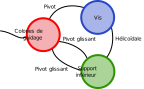
\includegraphics[width=.8\linewidth]{img/graphe_liaison.png}
\caption{\label{graphe_liaison}Graphe de liaisons}
\end{minipage}
\begin{minipage}{0.5\linewidth}
Soit le graphe des liaisons suivant :
\begin{itemize}
 \item $L_1$: encastrement,
 \item $L_2$: pivot d’axe $(E, \overrightarrow{z})$,
 \item $L_3$: pivot d’axe $(D, \overrightarrow{z})$,
 \item $L_4$: pivot d’axe $(F, \overrightarrow{z})$,
 \item $L_5$: pivot d’axe $(C, \overrightarrow{z})$,
 \item $L_6$: pivot d’axe $(B, \overrightarrow{z})$,
 \item $L_7$: pivot d’axe $(G, \overrightarrow{z})$,
 \item $L_8$: pivot d’axe $(H, \overrightarrow{z})$.
\end{itemize}
\end{minipage}
\end{figure}

\question{À l’aide de compositions des vitesses, écrire de 2 façons différentes $\overrightarrow{V_{C\in 3/1}}$.}


\question{À l’aide de compositions des vitesses de rotation, écrire de 2 façons différentes 
$\overrightarrow{\Omega_{3/1}}$.}

\question{À l’aide de compositions des torseurs, écrire de 2 façons différentes 
$\left\{ V_{3/1} \right\}$.}

\newpage

\section{La scie sauteuse}

On étudie ici une scie sauteuse dont le dessin de définition est donné dans le document réponse.

Le graphe de liaison et le schéma cinématique sont donnés sur les figures \ref{scie_liaisons} et \ref{scie_cin}.

\begin{figure}[ht!]
\begin{minipage}{0.45\linewidth}
   \def\svgwidth{\linewidth}
   \input{img/scie_liaisons.pdf_tex}
\caption{\label{scie_liaisons}Graphe de liaisons}
\end{minipage}\hfill
\begin{minipage}{0.45\linewidth}
   \def\svgwidth{0.75\linewidth}
   \input{img/scie_cin.pdf_tex}
\caption{\label{scie_cin}Schéma cinématique}
\end{minipage}
\end{figure}

Avec:
\begin{itemize}
 \item $\overrightarrow{AB}=-a\cdot\vec{x}+b\cdot\vec{y_1}$,
 \item $\overrightarrow{AC}=-c\cdot\vec{x}-d\cdot\vec{y}$,
 \item $\theta_1=(\vec{y},\vec{y_1})=(\vec{z},\vec{z_1})$,
 \item la vitesse de rotation de 1 par rapport à 0 est de $300\ tr\cdot min^{-1}$,
 \item les dimensions du mécanisme sont à mesurer sur le dessin d'ensemble.
\end{itemize}

\question{Colorier le dessin d'ensemble du document réponse pour faire apparaître les classes d'équivalence du mécanisme.}

\question{Déterminer le degré d'hyperstatisme du mécanisme à l'aide de la formule utilisant le nombre d'inconnues statiques du mécanisme.}

\question{Écrire les torseurs de toutes les liaisons du mécanisme en leur point d'application dans la base $R(\vec{x},\vec{y},\vec{z})$.}

\question{Écrire tous ces torseurs au point A dans la base $R(\vec{x},\vec{y},\vec{z})$.}

\question{Écrire le système d'équations issu de la fermeture cinématique du système.}

\question{Valider la valeur du degré d'hyperstatisme déterminé précédemment.}

\question{Déterminer l'expression des normes des vitesses de translation dans les liaisons $3/0$ et $3/2$ en fonction de $\omega_{x,10}$. Faire l'application numérique pour obtenir leurs valeurs maximales en $m\cdot s^{-1}$.}

\question{Les pièces 3 et 8 sont des coussinets en bronze, dont la vitesse de glissement maximale conseillée est $0.5\ m\cdot s^{-1}$. Leur utilisation est-elle compatible avec les résultats précédents ?}

\newpage

\section{Motoreducteur}

On s'intéresse maintenant au motoréducteur donc les vues éclatées et écorchées sont présentées sur les figures \ref{fig11} et \ref{fig12}. La nomenclature est fournie en fin de sujet et un plan à compléter est fourni en document réponse.

\begin{figure}[ht!]
\begin{center}
 \includegraphics[width=0.75\linewidth]{img/eclate}
  \caption{\label{fig11}Vue éclatée du motoréducteur}
  \includegraphics[width=0.75\linewidth]{img/ecorche}
  \caption{\label{fig12}Vue écorchée du motoréducteur}
  \end{center}
\end{figure}

\newpage

\question{A quoi correspond la pièce 6 ?}

\question{Donner le rapport de réduction du réducteur présent dans ce motoréducteur.}

\question{Colorier les classes d'équivalence du mécanisme (ne pas colorier à l'intérieur des ZONE 1 et ZONE 2).}

\question{Compléter la ZONE 1 en concevant une solution pour l'assemblage du pignon 10 avec le rotor 7. Vous pourrez utiliser la nomenclature afin de déterminer les pièces manquantes.}

\question{Compléter la ZONE 2 en concevant une solution pour l'assemblage du couvercle 3 sur le carter réducteur 2. Vous pourrez utiliser la nomenclature afin de déterminer les pièces manquantes.}

\finsujet

% Annexes
\includepdf[offset=15 -20]{img/nomenclature.pdf}

\debutcor

\reponse{4}{}{$\overrightarrow{V_{B\in 1/0}}=\overrightarrow{V_{A\in 1/0}}+\overrightarrow{BA}\wedge\overrightarrow{\Omega_{1/0}}$}

\reponse{4}{}{
$\left\{V\right\}=\left\{\begin{array}{cc}
\omega_x & 0\\0 & 0\\0&0
\end{array}
\right\}_A$}

\reponse{4}{}{$\overrightarrow{V_{C \in 3/1}}=\overrightarrow{V_{C\in 3/9}}+\overrightarrow{V_{C\in 9/8}}+\overrightarrow{V_{C \in 8/7}}+\overrightarrow{V_{C \in 7/1}}$

$\overrightarrow{V_{C \in 3/1}}=\overrightarrow{V_{C \in 3/9}}+\overrightarrow{V_{C \in 9/8}}+\overrightarrow{V_{C\in 8/10}}+\overrightarrow{V_{C \in 10/6}}+\overrightarrow{V_{C \in 6/1}}$}

\reponse{4}{}{$\overrightarrow{\Omega_{3/1}}=\overrightarrow{\Omega_{3/9}}+\overrightarrow{\Omega_{9/8}}+
\overrightarrow{\Omega_{8/7}}+\overrightarrow{\Omega_{7/1}}$

$\overrightarrow{\Omega_{3/1}}=\overrightarrow{\Omega_{3/9}}+\overrightarrow{\Omega_{9/8}}+
\overrightarrow{\Omega_{8/10}}+\overrightarrow{\Omega_{10/6}}+\overrightarrow{\Omega_{6/1}}$}

\reponse{4}{}{$\left\{V_{3/1}\right\}=\left\{V_{3/9}\right\}+\left\{V_{9/8}\right\}+
\left\{V_{8/7}\right\}+\left\{V_{7/1}\right\}$

$\left\{V_{3/1}\right\}=\left\{V_{3/9}\right\}+\left\{V_{9/8}\right\}+
\left\{V_{8/10}\right\}+\left\{V_{10/6}\right\}+\left\{V_{6/1}\right\}$}

\reponse{4}{\begin{center}
	\includegraphics[width=0.8\linewidth]{img/scie_vierge.png}
\end{center}}{\begin{center}
   \def\svgwidth{0.8\linewidth}
   \input{img/scie_cor.pdf_tex}
\end{center}}


\reponse{4}{}{$N_s=4+5+5+5=19$

$r_s=6\cdot(p-1)-m=6(4-1)-1=17$

$h=N_s-r_s=2$}

\reponse{4}{}{$\left\{V_{1/0}\right\}=\left\{\begin{array}{cc}
\omega_{x,10} & 0\\0 & 0\\0&0
\end{array}
\right\}_A$

$\left\{V_{2/1}\right\}=\left\{\begin{array}{cc}
\omega_{x,21} & 0\\0 & 0\\0&0
\end{array}
\right\}_B$

$\left\{V_{3/2}\right\}=\left\{\begin{array}{cc}
0 & 0\\0 & 0\\0&V_{z,32}
\end{array}
\right\}_A$

$\left\{V_{3/0}\right\}=\left\{\begin{array}{cc}
0 & 0\\\omega_{y,30} & V_{y,30}\\0&0
\end{array}
\right\}_C$}

\reponse{4}{}{$\overrightarrow{V_{A\in 2/1}}=\overrightarrow{V_{B\in 2/1}}+\overrightarrow{AB}\wedge\overrightarrow{\Omega_{2/1}}=(-a\cdot\vec{x}+b\cdot\vec{y_1})\wedge\omega_{x,21}\cdot\vec{x}=-b\cdot\omega_{x,21}\cdot\vec{z_1}$

$\overrightarrow{V_{A\in 2/1}}=-b\cdot\omega_{x,21}\cdot (-sin\theta_1\cdot\vec{y}+cos\theta_1\cdot\vec{z})$

$\left\{V_{2/1}\right\}=\left\{\begin{array}{cc}
\omega_{x,21} & 0\\0 & b\cdot\omega_{x,21}\cdot sin\theta_1\\0&-b\cdot\omega_{x,21}\cdot cos\theta_1
\end{array}
\right\}_A$

$\overrightarrow{V_{A\in 3/0}}=\overrightarrow{V_{C\in 3/0}}+\overrightarrow{AC}\wedge\overrightarrow{\Omega_{3/0}}=V_{y,30}\cdot\vec{y}+(-c\cdot\vec{x}-d\cdot\vec{y})\wedge\omega_{y,30}\cdot\vec{y}$

$\overrightarrow{V_{A\in 3/0}}=V_{y,30}\cdot\vec{y}-c\cdot\omega_{y,30}\cdot\vec{z}$

$\left\{V_{3/0}\right\}=\left\{\begin{array}{cc}
0 & 0\\\omega_{y,30} & V_{y,30}\\0&-c\cdot\omega_{y,30}
\end{array}
\right\}_A$}

\reponse{4}{}{$\left\{\begin{array}{l}
0=\omega_{x,21}+\omega_{x,10}\\
\omega_{y,30}=0\\
0=0+0\\
0=0+0\\
V_{y,30}=b\cdot\omega_{x,21}\cdot sin\theta_1\\
-c\cdot\omega_{y,30}=-b\cdot\omega_{x,21}\cdot cos\theta_1+V_{z,32}
\end{array}\right.$}

\reponse{4}{}{Il y a deux équations de la forme $0=0$, les autres sont indépendantes, donc $h=2$.}

\reponse{4}{}{$V_{y,30}=b\cdot\omega_{x,21}\cdot sin\theta_1=-b\cdot\omega_{x,10}\cdot sin\theta_1$

$V_{z,32}=b\cdot\omega_{x,21}\cdot cos\theta_1=-b\cdot\omega_{x,10}\cdot cos\theta_1$

$\omega_{x,10}=300\ tr\cdot min^{-1}=\dfrac{300\cdot 2\pi}{60}\ rad\cdot s^{-1}=10\cdot\pi\ rad\cdot s^{-1}=30 \ rad\cdot s^{-1}$

On mesure : $b=6\ mm=6\cdot 10^{-3}\ m$

$V_{y,30max}=-b\cdot\omega_{x,10}=6\cdot 10^{-3}\cdot 30=0.18\ m\cdot s^{-1}$

$V_{z,32max}=-b\cdot\omega_{x,10}=6\cdot 10^{-3}\cdot 30=0.18\ m\cdot s^{-1}$}

\reponse{4}{}{Oui car $0.18<0.5\ m\cdot s^{-1}$.}

\reponse{4}{}{Il est indiqué que c'est un ventilateur dans la nomenclature.}

\reponse{4}{}{$\dfrac{Z_{10}\cdot Z_8}{Z_{11}\cdot Z_{12}}=\dfrac{27\cdot 11}{45\cdot 67}\approx \dfrac{1}{5\cdot 2}\approx 0.1$
}

\ifdef{\public}{\includepdf[angle=90,offset=-20 -20]{img/Motoreducteur}}{\includepdf[angle=90,offset=-20 -20]{img/Motoreducteur_classes_equivalence.pdf}}
\ifdef{\public}{}{\includepdf[angle=90,offset=15 -20]{img/Motoreducteur_cor.pdf}}


\end{document}